\subsection{Model System}
To showcase the performance of RE-EDS, a system of five inhibitors (L1, L17, L19, L20 and L21) of checkpoint kinase 1 (CHK1) taken from Ref.~\cite{Huang2012} was chosen (Figure \ref{fig:Ligands/Protein}). The numbering of the compounds is according to Ref.~\cite{Huang2012}. The same system was studied in Ref.~\cite{Wang2017} as part of a series of scaffold hopping systems. Although the five ligands share a common substructure, they were considered to exemplify different types of core-hopping transformations (i.e. ring size change, ring opening/closing, ring extension) and R-group modifications \cite{Wang2017}.

\begin{figure}[h]
	\centering
	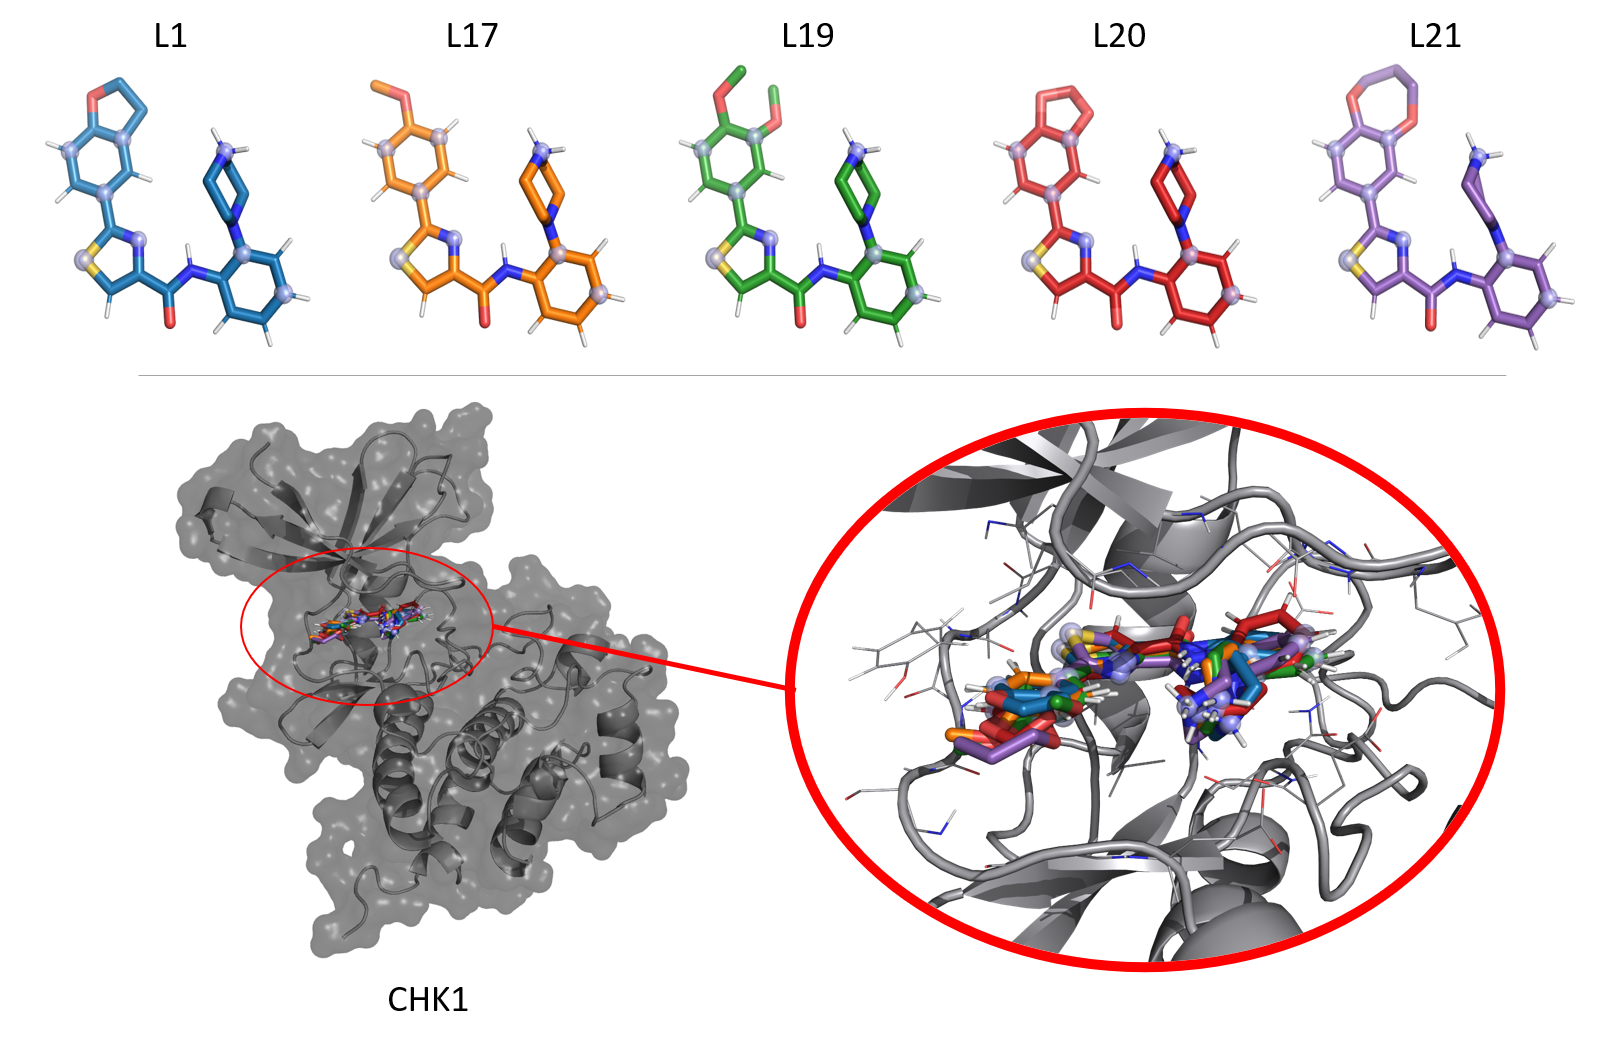
\includegraphics[width=\columnwidth]{fig/methods/CHK1_ring_opening_system_condense.png}
	\caption{(Top): 3D depiction of the five CHK1 inhibitors L1, L17, L19, L20, and L21 (numbering according to Ref.~\cite{Huang2012}). The selected locations of the distance restraints are indicated by the silver spheres. (Bottom): CHK1 protein in complex with the ligand bundle (PDB ID:3U9N).}
	\label{fig:Ligands/Protein}
\end{figure}

For the protein, the GROMOS 54A7 force field \cite{Schmid2011} was used. For the ligands, topologies were generated using the parametrization by the ATB server \cite{Mark2011} as an initial guess. The bonded terms were manually harmonized and adjusted to match the parameterization of similar functional groups in the GROMOS 54A7 force field. Partial charges were generated with our previous machine learning approach \cite{Bleiziffer2018} ($\epsilon$ = 4) and manually arranged into charge groups. The input files can be retrieved from: \\ https://github.com/rinikerlab/reeds/tree/main/examples/systems.

\subsection{System Preparation}%%initialize
The crystal structure of CHK1 in complex with ligand L1 (PDB ID:3U9N) was used as starting structure. The initial coordinates for ligands L17, L19, L20, L21 were generated with the {\tt{ConstrainedEmbed()}} functionality in the RDKit \cite{landrum2021}, where the common part was kept fixed in the crystal conformation. The coordinates of each ligand and those of the protein were subsequently energy minimized in vacuum using the steepest descent \cite{Ruder2016} approach implemented in the GROMOS software package \cite{Schmid2012}. 

%%build eds_system
A ``dual topology'' approach was used for the RE-EDS simulations, i.e. each ligand is present in the system separately \cite{Riniker2011}. Thus, each end state comprises of one active ligand and $N-1$ inactive (dummy) ligands. To avoid spatial drifting of the dummy ligands, eight distance restraints per ligand pair were defined within the common substructure (Figure \ref{fig:Ligands/Protein}) to connect all ligands in a ring with the help of the restraintmaker program (https://github.com/rinikerlab/restraintmaker) (order: -L1-L17-L19-L20-L21-). The reference distance was set to 0.0~nm and the force constant to $1000$~kJ~mol$^{-1}$~nm$^{-2}$.
The combined topology file was generated with the program {\tt{prep\_eds}} in the GROMOS++ \cite{eichenberger2011} package. 
The EDS system was solvated in a cubic box of single-point-charge (SPC) \cite{Berendsen1981} water (resulting in 1'848 solvent molecules for the ligands in water and 15'639 solvent molecules for the protein-ligands complex). 
An energy minimization was carried out with the steepest descent algorithm \cite{Ruder2016}, where all solute atoms were position restrained with a force constant of $25'000$~kJ~mol$^{-1}$~nm$^{-2}$. 

\subsection{Simulation Details}
All simulations were performed with the GROMOS software package \cite{Schmid2012} (freely available on http://www.gromos.net).
The equilibrations and production runs were carried out under isothermal-isobaric (NPT) conditions using the leap-frog integration algorithm \cite{Hockney1970} and a time step of $2$~fs. 
Bond lengths were constrained with SHAKE \cite{ryckaert1977} using a tolerance of $10^{-4}$. 
The nonbonded contributions were calculated with a twin-range scheme using a short-range cutoff of $0.8$~nm and a long-range cutoff of $1.4$~nm. 
The electrostatic nonbonded contributions beyond the long-range cutoff were calculated with the reaction-field \cite{tironi1995} approach and a dielectric permittivity of 66.7 \cite{Glattli2002} for water. 
The temperature was kept constant at $300$~K using the weak coupling scheme \cite{Berendsen1984} and a coupling time of $0.1$~ps$^{-1}$. The pressure was kept at $1.031$~bar ($1$~atm) with the same type of algorithm and a coupling time of $0.5$~ps$^{-1}$ and an isothermal compressibility of $4.575 \cdot 10^{-4}$~(kJ~mol$^{-1}$~nm$^{-3}$)$^{-1}$.
Rotation and translation of the center of mass of the simulation box were removed every $2$~ps. 
Energies were written to file every $20$ steps and coordinates every $5'000$ steps.
In the RE-EDS simulations, replica exchanges was attempted every $20$ steps.

\subsection{RE-EDS Workflow}
The Python code to manage the RE-EDS workflow, including the analysis steps, can be retrieved from: https://github.com/rinikerlab/reeds.
The workflow starts with the energy-minimized coordinates of the EDS system (all $N$ ligands plus environment, dominating end state is L20) into the parameter exploration step, which is used as equilibration phase.
A RE-EDS simulation of 0.2~ns length was performed with 21 logarithmically distributed replicas between $s=1.0$ and $10^{-5}$ and all energy offsets set to zero.  
The thresholds $T_{i}^{\text{us}}$ were estimated from replicas with very low $s$-values.
Undersampling was observed when each end state occurred with a fraction $f_{i}^{\text{occur,us}} \ge 0.75$ during the simulation period.
To be conservative, the lower bound of the $s$-parameters for the following steps was set to the $s$-value two levels below the highest replica with undersampling.

To optimize the coordinates of the system for each end state, an EDS simulation of 0.2~ns length was performed for each end state $i$ with $s=1.0$ and $E^R_i=500$~kJ~mol$^{-1}$ while the energy offsets of all other end states were set to $-500$~kJ~mol$^{-1}$. L20 was the initial dominating end state in the starting configuration. 
The coordinates were considered to be optimized when the desired end state was constantly sampled as the dominating state in the last 30~\% of the simulation. 

%param optimization
%%Eoff
To determine the energy offsets, a 1.2~ns RE-EDS simulation was carried out with 21 logarithmically distributed replicas between $s=1.0$ and the lower bound (determined above). The first 0.4~ns of the simulation were discarded as equilibration. This simulation was performed in two manners: (i) using the final coordinates from the lower-bound determination as starting configuration for all replicas (1SS approach), or (ii) using the different optimized coordinates from the previous substep for the replicas in an alternating way (SSM approach). 
For the PEOE \cite{Sidler2016} scheme, the following parameters were used: fraction $f_{i}^{\text{us}} \ge 0.9$ and the potential thresholds determined in the lower bound exploration $T_{i}^{\text{us}}$.

%%S-opt
The iterative optimization of the $s$-distribution with the N-LRTO \cite{Sidler2017} algorithm was started with the energy offsets and the final coordinates of the previous substep.
Four replicas were added per iteration. 
The simulation length of the first iteration was $0.4$~ns, and subsequently increased by $0.4$~ns at each iteration until a maximum length of $1.2$~ns was reached.
The $s$-distribution was considered converged if all end states were sampled as dominating states during the RE-EDS simulation at $s=1.0$ and the improvement of the round-trip time was below $\Delta \tau < 5$~ps.

The production run with constant reference-state parameters was performed for $4$~ns.

\subsection{Simulation of Single States}
The input coordinates for the simulations of the individual end states were extracted from the RE-EDS starting coordinates and subsequently energy minimized. Next, a production run of $4$~ns was performed. 

\subsection{Analysis}
Free-energy differences were calculated with the program {\tt{dfmult}} from the \textit{GROMOS++} \cite{eichenberger2011} package.
Statistical analysis and handling of the workflow steps are based on the Python packages pandas \cite{Mckinney2010}, Matplotlib \cite{Hunter2007}, NumPy \cite{VanDerWalt2011}, SciPy \cite{Virtanen2020}, and PyGromosTools \cite{ries2021}.